
%(BEGIN_QUESTION)
% Copyright 2012, Tony R. Kuphaldt, released under the Creative Commons Attribution License (v 1.0)
% This means you may do almost anything with this work of mine, so long as you give me proper credit

A very common form of schematic used to represent large-scale electric power systems is the {\it single-line diagram}, where all three phase conductors in a circuit are represented by single lines in the diagram.  A single-line diagram showing a power plant sending power to a substation for distribution to business and residential loads is shown here:

$$\includegraphics[width=15.5cm]{i02116x01.eps}$$

A concern in electric power grids is {\it breaker failure}: when a circuit breaker fails to open as it should when given a ``trip'' signal.  Suppose breaker \#5 fails to open all its contacts when manually tripped.

Identify which other substation breakers must be tripped in order to isolate the failed breaker \#5 from all power, after the breaker failure has been detected by a ``breaker failure'' relay monitoring breaker \#5.  How many loads (power customers) are affected by this subsequent action?

\vskip 10pt

\filbreak

Suppose the PFD for each of breaker \#5's three power contacts is 0.000273.  Calculate the probability of {\it any} of these contacts failing to open when the breaker mechanism is tripped.

\vskip 10pt

Also, how do you think a breaker failure might be detected by electronic devices?  What diagnostic data would a breaker-failure detection circuit ``look for'' in order to determine a breaker had indeed failed to open all its contacts when tripped?  Examine this photograph of a 125 kV SF$_{6}$ gas circuit breaker for clues:

$$\epsfxsize=4in \includegraphics[width=15.5cm]{i02116x02.eps}$$

\vskip 20pt \vbox{\hrule \hbox{\strut \vrule{} {\bf Suggestions for Socratic discussion} \vrule} \hrule}

\begin{itemize}
\item{} Why do you suppose single-line diagrams are popular within the electrical power industry, rather than full schematic diagrams showing all power conductors?
\item{} What would happen in this power system if breaker ``F'' were to trip?
\item{} Suppose the dependability of each breaker in this system (i.e. the probability it will trip when called to trip) is 0.99918, and the security of each breaker in this system (i.e. the probability it won't trip when it's not supposed to) is 0.99993.  Based on these figures, calculate the following probabilities:
\begin{itemize}

\item{} The probability that the left-hand transmission line will be unnecessarily removed from service (i.e. opened so it no longer carries load current).
\item{} The probability that one particular generator will be taken off-line unnecessarily.
\item{} The probability that {\it any} of the generators will be taken off-line unnecessarily.
\item{} The probability that the high-voltage bus cannot be isolated in the event of a fault.
\item{} The probability that the left-hand substation bus cannot be isolated in the event of a fault.
\item{} The probability that the left-hand substation bus will become unnecessarily isolated.
\item{} The probability that the entire substation will suffer an unnecessary outage.
\end{itemize}
\end{itemize}

\underbar{file i02116}
%(END_QUESTION)





%(BEGIN_ANSWER)

PFD = 0.000818776

\vskip 10pt

One way to detect a failed breaker is by monitoring the current through it in the ``tripped'' state.  Obviously, a tripped circuit breaker should have no current going through its contacts at all!  The question now becomes, how to measure current through the circuit breaker, and this is where the photo proves its value: the numbered cylinders at the base of each insulator bushing on the circuit breaker each houses one current transformer (CT).  This is standard on high-voltage circuit breaker construction: each terminal into and out of the circuit breaker has its own dedicated CT to be used for current monitoring, and these current signals may be used to detect a failed breaker condition.

%(END_ANSWER)





%(BEGIN_NOTES)

After a failure has been detected in breaker \#5, the following circuit breakers need to be tripped in order to isolate breaker \#5:

\begin{itemize}
\item{} Breakers \#1, \#2, \#3, and \#4 (isolates Bus A from all power sources)
\item{} Breaker \#10 (isolates breaker \#5 from Bus B)
\end{itemize}

This protective action cuts power to all loads on the bottom distribution line, while maintaining power (from Bus B) to all other loads.

\vskip 10pt

PFD calculation:

$$\includegraphics[width=15.5cm]{i02116x03.eps}$$

\vfil \eject

The Socratic Questions on probability may be answered by first organizing the given information on breaker dependability and security (as well as the complementary measures of undependabilty (PFD) and unsecurity, shown in italic font):

% No blank lines allowed between lines of an \halign structure!
% I use comments (%) instead, so that TeX doesn't choke.

$$\vbox{\offinterlineskip
\halign{\strut
\vrule \quad\hfil # \ \hfil & 
\vrule \quad\hfil # \ \hfil & 
\vrule \quad\hfil # \ \hfil \vrule \cr
\noalign{\hrule}
%
% First row
& {\bf Breaker told to trip} & {\bf Breaker not told to trip} \cr
%
\noalign{\hrule}
%
% Another row
{\bf Breaker trips} & 0.99918 & {\it 0.00007} \cr
%
\noalign{\hrule}
%
% Another row
{\bf Breaker does not trip} & {\it 0.00082} & 0.99993 \cr
%
\noalign{\hrule}
} % End of \halign 
}$$ % End of \vbox

In general terms, this is what each of the cells in the table mean:

% No blank lines allowed between lines of an \halign structure!
% I use comments (%) instead, so that TeX doesn't choke.

$$\vbox{\offinterlineskip
\halign{\strut
\vrule \quad\hfil # \ \hfil & 
\vrule \quad\hfil # \ \hfil & 
\vrule \quad\hfil # \ \hfil \vrule \cr
\noalign{\hrule}
%
% First row
& {\bf Breaker told to trip} & {\bf Breaker not told to trip} \cr
%
\noalign{\hrule}
%
% Another row
{\bf Breaker trips} & Dependability (RSA) & Un-security \cr
%
\noalign{\hrule}
%
% Another row
{\bf Breaker does not trip} & Un-dependability (PFD) & Security \cr
%
\noalign{\hrule}
} % End of \halign 
}$$ % End of \vbox



Any given scenario may then be drawn as a logic gate diagram with appropriate values pulled from the table:

\begin{itemize}
\item{} The probability that the left-hand transmission line will be unnecessarily removed from service (i.e. opened so it no longer carries load current).  {\it (i.e. the probability that either breaker G or J or 1 will trip when it's not supposed to.)}
\end{itemize}
\end{itemize}

$$\includegraphics[width=15.5cm]{i02116x04.eps}$$

















\vfil \eject

\noindent
{\bf Summary Quiz:}

Suppose circuit breaker \#7 fails to open when it is commanded to trip.  Which breakers should be tripped in order to isolate the failed breaker \#7 from all power while maintaing power to as many loads as possible?

$$\includegraphics[width=15.5cm]{i02116x01.eps}$$

\begin{itemize}
\item{} 6, 8, and 11
\vskip 5pt 
\item{} 1, 2, 3, and 6
\vskip 5pt 
\item{} 3, 6, 8, and 11
\vskip 5pt 
\item{} 3, 6, 8, and 9
\vskip 5pt 
\item{} 3, 6, 11, and 12
\vskip 5pt 
\item{} A and B
\end{itemize}


















\vfil \eject

\noindent
{\bf Summary Quiz:}

Suppose a phase-to-phase fault develops on one of the loads fed from the top distribution bus in the substation.  Which breakers should be tripped in order to isolate that faulted load from all power while maintaing power to as many loads as possible?

$$\includegraphics[width=15.5cm]{i02116x01.eps}$$


%INDEX% Electric power systems: HV circuit breaker controls (breaker failure)
%INDEX% Electric power systems: single-line diagram

%(END_NOTES)


